\documentclass{tudelft-report}

%% We need to increase the paper size to slightly larger than twice A4 to make
%% room for a front and back cover, including the spine.


\usepackage{fancyhdr}
\usepackage{lipsum}

\usepackage{float}

%Tikz related libraries goes here
\usepackage{tikz}           % Draw beautiful vector images
\usepackage{tikz-3dplot}
\usepackage{fontawesome}    % Beautiful and free icons

\usetikzlibrary{shapes.geometric, arrows}

\usetikzlibrary{angles}
\usetikzlibrary{quotes}
\usetikzlibrary{arrows.meta}
\usetikzlibrary{positioning}
\usetikzlibrary{automata}
\usetikzlibrary{decorations.pathreplacing}
\usetikzlibrary{patterns}   % https://tex.stackexchange.com/questions/29359/pgfplots-how-to-fill-the-area-under-a-curve-with-oblique-lines-hatching-as-a
\usetikzlibrary{calc}       % Used to draw beautiful molecules out of atoms in Appendix

\usepackage{listings}       % Lstlisting code viewer

\usepackage{longtable}      % Multipage tables

\addtolength{\headheight}{0.9cm} % make more space for the header
\pagestyle{fancyplain} % use fancy for all pages except chapter start
\lfoot{
\includegraphics[height=1.3cm]{figures/colortudelft.png}} % left logo
\rhead{
\includegraphics[height=1.3cm]{figures/projectluna.png}} % right logo
\renewcommand{\headrulewidth}{0pt} % remove rule below header

\setlength\parindent{0pt}       % Do not indent a new paragraph

\def\iic{\texorpdfstring{I$^2$C}{I2C}}  % I2C text format


\definecolor{darkpink}{rgb}{1.0, 0.13, 0.32}
\definecolor{mGreen}{rgb}{0,0.6,0}                      %C style lstlisting
\definecolor{mGray}{rgb}{0.5,0.5,0.5}                   %C style lstlisting
\definecolor{mPurple}{rgb}{0.58,0,0.82}                 %C style lstlisting
\definecolor{backgroundColour}{rgb}{0.95,0.95,0.92}     %C style lstlisting


\lstdefinestyle{DOS}
{
    backgroundcolor=\color{black},
    basicstyle=\scriptsize\color{white}\ttfamily
}

\lstdefinestyle{CStyle}{
    backgroundcolor=\color{backgroundColour},
    commentstyle=\color{mGreen},
    keywordstyle=\color{magenta},
    numberstyle=\tiny\color{mGray},
    stringstyle=\color{mPurple},
    basicstyle=\footnotesize,
    breakatwhitespace=false,
    breaklines=true,
    captionpos=b,
    keepspaces=true,
    numbers=left,
    numbersep=5pt,
    showspaces=false,
    showstringspaces=false,
    showtabs=false,
    tabsize=2,
    language=C
}

% Define TikZ flow diagram blocks here
\tikzstyle{startstop} = [rectangle, rounded corners, minimum width=3cm, minimum height=1cm,text centered, draw=black, fill=red!30]
\tikzstyle{io} = [trapezium, trapezium left angle=70, trapezium right angle=110, minimum width=3cm, minimum height=1cm, text centered, draw=black, fill=blue!30]
\tikzstyle{process} = [rectangle, minimum width=3cm, minimum height=1cm, text centered, draw=black, fill=orange!30]
\tikzstyle{decision} = [diamond, minimum width=3cm, minimum height=1cm, text centered, draw=black, fill=green!30]
\tikzstyle{arrow} = [thick,->,>=stealth]

\begin{document}
%% Use Roman numerals for the page numbers of the title pages and table of
%% contents.
% \frontmatter

%% Uncomment following 19 lines for a cover with a picture on the lower half only
\title[tudelft-white]{Serial library}
\subtitle[tudelft-cyan]{Lunar Zebro}
\author[tudelft-white]{Software Department}
\affiliation{-}
\coverimage{figures/page1background.png}
\titleoffsetx{2cm}
\titleoffsety{8cm}
\afiloffsetx{1cm}
\afiloffsety{18cm}
\covertext[tudelft-white]{
    \textbf{Cover Text} \\
    possibly \\
    spanning
    multiple
    lines
    \vfill
    ISBN 000-00-0000-000-0
}
\setpagecolor{black}
\makecover



%
%% Include an optional title page.
\begin{titlepage}


\begin{center}

%% Insert the TU Delft logo at the bottom of the page.

%% Print the title in cyan.
{\makeatletter
\largetitlestyle\fontsize{64}{94}\selectfont\@title
%\largetitlestyle\color{tudelft-cyan}\Huge\@title
\makeatother}

%% Print the optional subtitle in black.
{\makeatletter
\ifx\@subtitle\undefined\else
    \bigskip
   {\tudsffamily\fontsize{22}{32}\selectfont\@subtitle}
    %\titlefont\titleshape\LARGE\@subtitle
\fi
\makeatother}

\bigskip
\bigskip

by
%door

\bigskip
\bigskip

%% Print the name of the author.
{\makeatletter
%\largetitlefont\Large\bfseries\@author
\largetitlestyle\fontsize{26}{26}\selectfont\@author
\makeatother}

\bigskip
\bigskip

in partial fulfilment of the requirements for documentation for:
%ter verkrijging van de graad van Master of Science

TU Delft, The Netherlands
%aan de Technische Universiteit Delft,

%to be defended publicly on Tuesday January 1, 2013 at 10:00 AM.
%in het openbaar de verdedigen op dinsdag 1 januari om 10:00 uur.

\vfill

\begin{tabular}{lll}
    Project Director: & prof. dr. ir. C. J. M. Verhoeven, & TU Delft \\
    System Engineer: & Pranav Gurumallappa, & TU Delft \\
    Operations Manager: & Maneesh Verma, & TU Delft \\
%    Project duration: & \multicolumn{2}{l}{March 1, 2012 -- January 1, 2013} \\
    Head of Software: & dr. A. Noroozi, & TU Delft \\
    Vice Head of Software: & Y. Klaassens, & TU Delft \\
\end{tabular}
%% Only include the following lines if confidentiality is applicable.

\bigskip
\bigskip
\emph{This document is confidential and cannot be made public unless a written permission has been obtained from project director.
}
%\emph{Op dit verslag is geheimhouding van toepassing tot en met 31 december 2013.}

\bigskip
\bigskip
%An electronic version of this thesis is available at %\url{http://repository.tudelft.nl/}.
%\\[1cm]

%\centering{
\includegraphics{cover/logo_black}}


\end{center}

\begin{tikzpicture}[remember picture, overlay]
    \node at (current page.south)[anchor=south,inner sep=0pt]{
        
\includegraphics{cover/logo_black}
    };
\end{tikzpicture}

\end{titlepage}


\tableofcontents

%% Use Arabic numerals for the page numbers of the chapters.
% \mainmatter

\chapter{Introduction}
Because RS485 is a half-duplex protocol, software on both ends of the physical data line should follow the same set of rules defined in the protocol and Message Format (see Chapter \ref{ch:message_format}). The Bus Manager is responsible for transferring commands and data between subsystems while adhering to this format.
This implies checking for CRC errors and sending a retransmission request or NACK when it needs to do so.
The Bus Manager acts between the Application Layer and the Physical Layer of the OSI model.

Figure \ref{fig:rs485_diagram} shows that there are 5 different RS485 buses inside the rover.
The Bus Manager also prevents any race condition on its assigned bus and makes sure that multiple apps cannot communicate with their subsystem at the same time.
\todo[inline]{Not sure about this yet}

\begin{figure}[H]
    \centering
    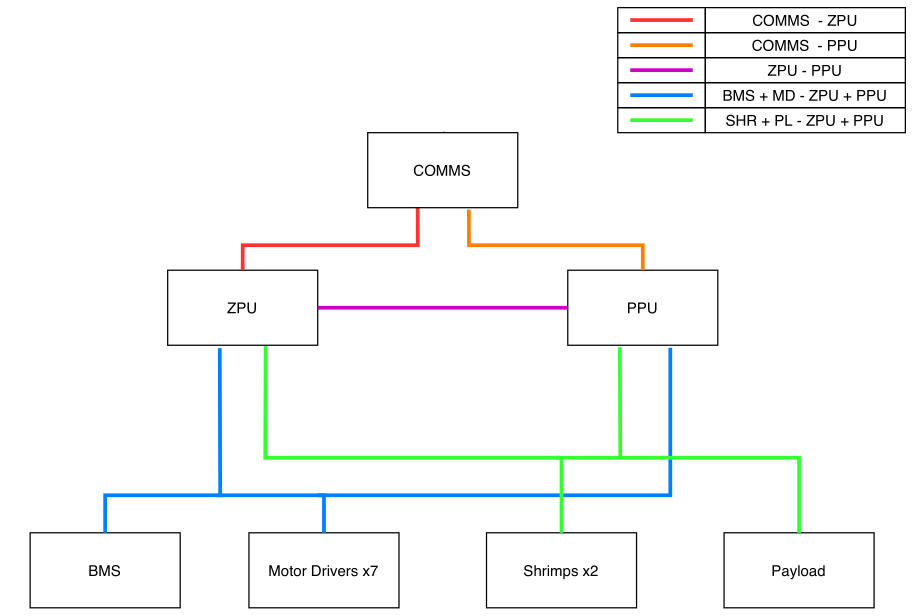
\includegraphics[scale=0.4]{figures/RS485_connections.png}
    \caption{Schematic view of the physical RS485 busses layout}
    \label{fig:rs485_diagram}
\end{figure}


\newpage


It is a bit awkward and impractical to uniquely identify RS485 buses based on the colours used in Figure \ref{fig:rs485_diagram}.
This is why we map the colours of Figure \ref{fig:rs485_diagram} to a unique bus name and number.
Table \ref{tab:buslegend} shows this mapping.
From now on in this document as well as in code, we will refer to bus names rather than bus colours.

\definecolor{amethyst}{rgb}{0.6, 0.4, 0.8}
\definecolor{bleudefrance}{rgb}{0.19, 0.55, 0.91}

\begin{longtable}{| p{0.1\textwidth} | p{0.15\textwidth} | }
    \hline
    \textcolor{red}{Bus name} & \textcolor{red}{Bus colour} \\
    \hline
    Bus0 & 
\begin{tikzpicture} \draw[line width=1mm, color=red] (0,0) -- (2,0); \end{tikzpicture} \\
    \hline
    Bus1 & 
\begin{tikzpicture} \draw[line width=1mm, color=orange] (0,0) -- (2,0); \end{tikzpicture} \\
    \hline
    Bus2 & \begin{tikzpicture} \draw[line width=1mm, color=amethyst] (0,0) -- (2,0); \end{tikzpicture} \\
    \hline
    Bus3 & \begin{tikzpicture} \draw[line width=1mm, color=bleudefrance] (0,0) -- (2,0); \end{tikzpicture} \\
    \hline
    Bus4 & 
\begin{tikzpicture} \draw[line width=1mm, color=green] (0,0) -- (2,0); \end{tikzpicture} \\
    \hline

    \caption{Bus legend mapping bus names to colours}
    \label{tab:buslegend}
\end{longtable}


\section{Background information and History}

\subsection{First version (1.0)}
Bus Manager is a concept that was first introduced in February 2021 as part of Max' thesis \cite{comms_thesis}.
Between February 2021 and August of 2021, the foundational layer of Bus Manager was laid which includes, but is not limited to, the Message Format.
Unit tests have shown that this first revision of Bus Manager used to work.

\subsection{Second version (2.0)}
In the second revision of Bus Manager, a few modifications have been made.
One of these changes is, for instance, that the Bus Manager won't send an initial message to request if an $x$ amount of bytes are available for the receiver to receive. Instead, it will just send the command which includes the length as part of the Message Format.
\todo[inline]{Clear up this sentence}
\par The second revision also uses a semaphore to synchronise bus access between bus managers, because the idea was for each subsystem app to have its own bus manager.

\subsection{Third version (2.1)}
The third version of the Bus Manager uses a more centralised approach. The Bus Managers live on the OBC in their own app, which coordinates bus access for all buses. Apps need to communicate with the Bus Managers via inter-thread communication. This avoids the need for using shared semaphores and decreases the dependencies between the subsystem apps. For further information about the design, see Chapter \ref{ch:design}.


\section{List of features of Bus Manager 2.1}

Now that the reader is aware of the overall functionality of the Bus Manager, we can list a set of features that characterises Bus Manager 2.1 (subject to change).

\begin{itemize}

    \item{\textbf{Instances}. Each bus has a separate instance of the Bus Manager that manages the access to that bus. Avoids the need for a more complex solution for all buses.}

    \item{\textbf{Timeout}. When a Bus Manager sends any type of message it waits for a response. A configurable timeout limit can be set to signal an error if the response is not received within that limit. }

    \item{\textbf{Retries}. When too many timeouts have happened and \textbf{<tbd>} retries are exceeded, then the application layer of this particular Bus Manager is informed about the failure.}

    \item{\textbf{Portability}. Because of the extensive use of Bus Manager both on the masters (OBC, PPU) and slaves (subsystems), it is of extra interest to design and implement Bus Mananger in such a way that it is easy to port over to subsystems which run different hardware architectures. Reimplementing it means that subsystem designers need to be fully aware of the protocol- and Message Format and this is a source of error and requires extra testing and validating. Bus Manager should be easily portable and be abstract in nature.}

    \item{\textbf{Sustainability}. Bus Manager shall comply to the Lunar Zebro Software guidelines. These include, but are not limited to: the code style guide and GoogleTest Unit Tests. The Git repository follows the same skeleton as all the other software modules.}

\end{itemize}


\chapter{Software Design}

This section highlights the Software Design by providing an overview of both
the Serial library as well as the MSP-Serial library. Diagrams and design
decisions will be shown and elaborated here.

\section{Serial}

The Serial library offers three major components which are configuring, writing
and reading. Lets go over each one of them and explain in further detail how
that looks like 

\subsection{Configuring a File Descriptor}

In Linux or any Unix-like operating system, file descriptors have to be
configured. The Serial library offers some level of flexibility in terms of
options to configure like blocking (return until all bytes have been send or
return until something has been read) or non-blocking mode, the baudrate of the
file descriptor and more. There is also some device-specific settings like physical I/O
pins that needs to be configured. The Serial library uses the Linux RS-485
kernel module because toggling the RS-485 DE pin in software turned out to be
too slow (See Appendix entry in Subsection \ref{subsec:de-bug}).

\begin{figure}[H]
\centering
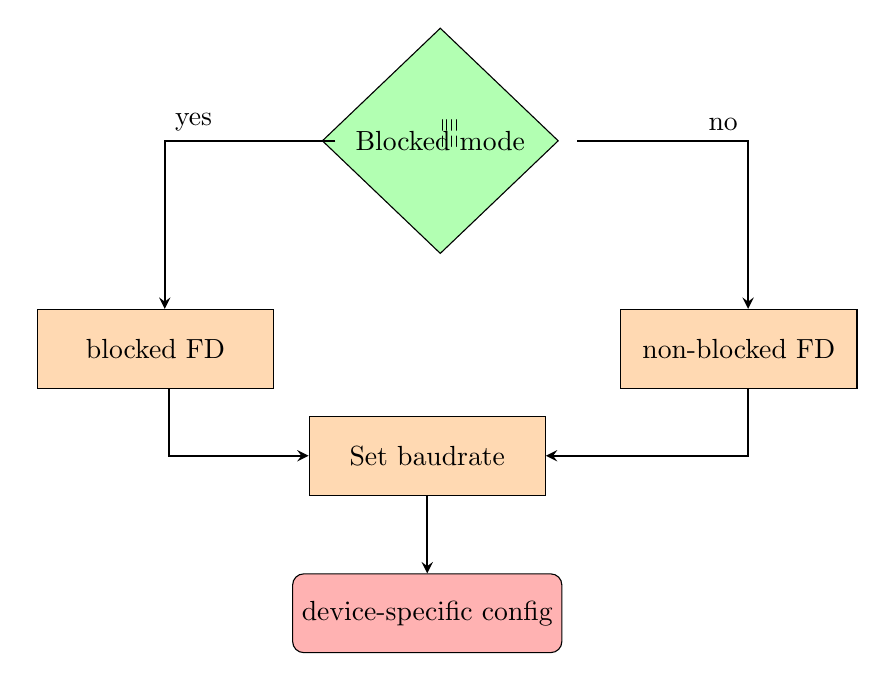
\begin{tikzpicture}[node distance=2cm, scale=1, transform shape]

    ¦   \node (decision1) [decision, align=center] {Blocked mode};
    ¦   \node (process1) [process, below left=of decision1, align=center] {blocked FD};
    ¦   \node (process2) [process, below right=of decision1, align=center] {non-blocked FD};

    ¦   \draw [arrow] (decision1) -| node [anchor=south west] {yes} (process1);
    ¦   \draw [arrow] (decision1) -| node [anchor=south east] {no} (process2);

        \node (process3) [process, below of=decision1, xshift=-0.4cm, yshift=-2cm, align=center] {Set baudrate};

        \draw [arrow] (process1) |- node [anchor=south west] {} (process3);
        \draw [arrow] (process2) |- node [anchor=south west] {} (process3);

        \node (stop) [startstop, below of=process3, align=center] {device-specific config};
        
        \draw [arrow] (process3) -- node [anchor=south west] {} (stop);


\end{tikzpicture}

\caption{Flow-chart showing the high-level overview of configuring a file descriptor}
\label{fig:serialsocketconfig}

\end{figure}

\newpage
\subsection{Writing}

Writing is fairly easy as it uses the file descriptor to write to the file descriptor
whatever data and length is given.  This means that it is the responsibility of
the user of the Serial library to make sure that no write-overflow will happen
(length is greater than the amount of bytes to write).

\subsection{Reading}
TODO after bug is fixed.

\newpage
\section{MSP-Serial}

The MSP430FR5969 microcontroller has two eUSCI peripherals, namely eUSCI\_A0
and eUSCI\_A1 which can and will be configured to be in UART mode. Each UART
peripheral will be wired to an RS-485 transceiver and hooked to a RS-485 bus.
COMMs is the only exception compared to the rest of the subsystems as it will
have full-duplex RS-485 communication to the OBC. \newline

\subsection{Configuration and setting up}

The first step is configuring the I/O pin and the eUSCI\_$ \text{A}_x$
peripheral attached to the pin. This is shown in Figure
\ref{fig:mspuartconfig}. As of now, the baudrate is configured to be 115200. 

\begin{figure}[H]
\centering
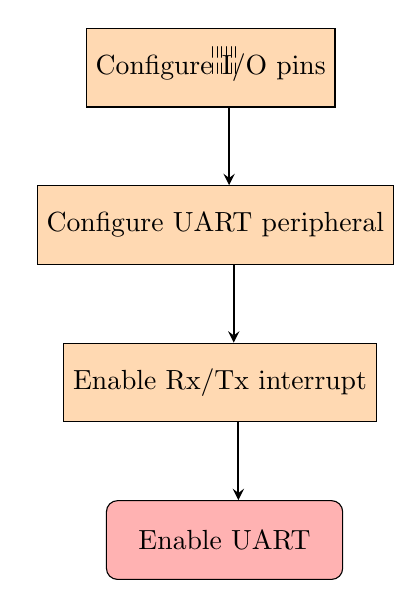
\begin{tikzpicture}[node distance=2cm, scale=1, transform shape]

    ¦   \node (process1) [process, align=center] {Configure I/O pins};
    ¦   \node (process2) [process, below of=process1, align=center] {Configure UART peripheral};
    ¦   \node (process3) [process, below of=process2, align=center] {Enable Rx/Tx interrupt};
    ¦   \node (process4) [startstop, below of=process3, align=center] {Enable UART};


    ¦   \draw [arrow] (process1) -- node [anchor=south west] {} (process2);
    ¦   \draw [arrow] (process2) -- node [anchor=south west] {} (process3);
    ¦   \draw [arrow] (process3) -- node [anchor=south west] {} (process4);

\end{tikzpicture}

\caption{Flow-chart showing the high-level overview of configuring a UART
    peripheral}
\label{fig:mspuartconfig}

\end{figure}

\subsection{Writing}

Writing is fairly easy. Data is written to the UCAxTXBUF register in
a busy-wait fashion. 

\subsection{Reading}

The biggest design is contained in the reading off Serial. That is because the
MSP430 will receive an arbitrary amount of bytes and we need to buffer them.
The Bus Manager can determine how many bytes will be received but that is part
of the Lunar Zebro Bus Manager protocol. After all, after receiving all bytes
the CRC can be calculated and it can be validated if the packet is valid. But
before all of that has happened in the Bus Manager, the MSP-Serial library
needs to have received all the bytes. \newline

The Interrupt-Service-Routine (ISR) is used to read a single byte from the UART
peripheral and buffered. A state-machine is used as well as a timeout.

%TODO: Add the UML state diagram


\chapter{Usage and API}


\chapter{Appendix}

\section{Known bugs and issues}

This section will list all known bugs and issues encountered during the development of the firmware.


\section{Fixed bugs and issues}

\subsection{Switching the \texttt{DE} pin seems inaccurate on higher speeds on the Raspberry Pi Zero2}
\label{subsec:de-bug}

This issue has been discovered on the Raspberry Pi Zero 2 which is used on the Test Setup V1.1 and has to do with toggling the \texttt{DE} pin of the RS-485 transceiver when the RPI wants to send data to the bus.
Serial uses a calculation to determine how long it should wait until the \texttt{DE} pin can be toggled from writing (1) back to reading (0) which is shown below in Listing \ref{lst:serial_write_delay}.

\begin{lstlisting}[frame=single, caption={Dynamic calculated sleep depending on length of data and baudrate}, captionpos=b, label={lst:serial_write_delay}, basicstyle=\small, style=CStyle]
     int time_to_sleep = (((float) length) / (float) ((float) baud / 10.0)) * 1000000.0;
\end{lstlisting}

The baudrate is the amount of bits that are send. Since we send 10 bits per byte (8 data bits, a start bit and a stop bit) we divide the baudrate by 10 to get the amount of bytes per second.
The total length of the data divided by the bytes per second leaves a delay expressed in seconds. Since we want some level of accuracy, we multiply it by a million and use the \texttt{usleep()} function.
When we test this formula on a baudrate of 9600 we can see that the \texttt{DE} pin is toggled right after the last bit is send. This can be seen in Figure \ref{fig:scope_no_extra_delay}.


\begin{figure}[H]
    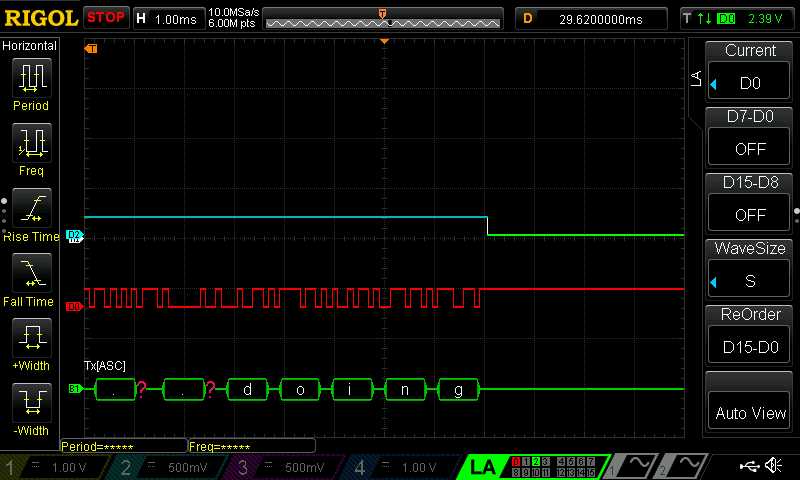
\includegraphics[scale=0.4]{figures/Scope_No_Extra_Delay.png}
    \caption{Baudrate 9600 and using the formula in Listing \ref{lst:serial_write_delay}, everything seems fine. \texttt{D2} is RS485 DE pin and \texttt{D0} is the TX pin}
    \label{fig:scope_no_extra_delay}
\end{figure}


\newpage
Because the Operating System on the RPI where this software is tested on, it might be safe to add a bit of extra timing in order to make sure that the data is on the bus. For instance, we could add 1 to \texttt{length} in Listing \ref{lst:serial_write_delay} to wait for an extra byte delay.
When we do so and send again on 9600 baud, we should expect a little above ~1.04 milliseconds extra delay before the \texttt{DE} pin is toggled.
This can be seen in Figure \ref{fig:scope_extra_delay9600} where the division is set to 1 millisecond. Indeed, the \texttt{DE} pin is toggled a little after ~1.04 milliseconds.

\begin{figure}[H]
    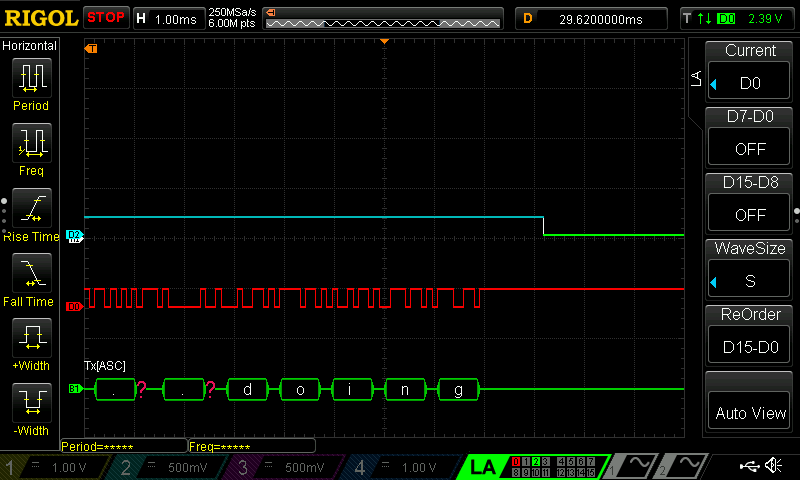
\includegraphics[scale=0.4]{figures/Scope_Extra_Delay9600.png}
    \caption{Baudrate 9600 and using the formula in Listing \ref{lst:serial_write_delay} but added 1 to \texttt{length}}
    \label{fig:scope_extra_delay9600}
\end{figure}

However, things start to get wacky on higher baudrates such as 115200.
In the example in Figure \ref{fig:scope_no_delay115200} we are sending 30 bytes.
This means we will sleep for $\frac{30}{11520} * 1000000 = 2604  \mu S$.
We can see that the \texttt{DE} pin stays up for \texttildelow3100 $\mu S$ without adding any extra delay in the formula in Listing \ref{lst:serial_write_delay} while the data seems to be okay but a bit on the higher end of the time spectrum.
The reason for this extra time could be that the \texttt{usleep()} tells the Operating Systems that this process can be unblocked now, but perhaps another process on the CPU is running now. Hence the extra time delay that is unwanted.


\begin{figure}[H]
    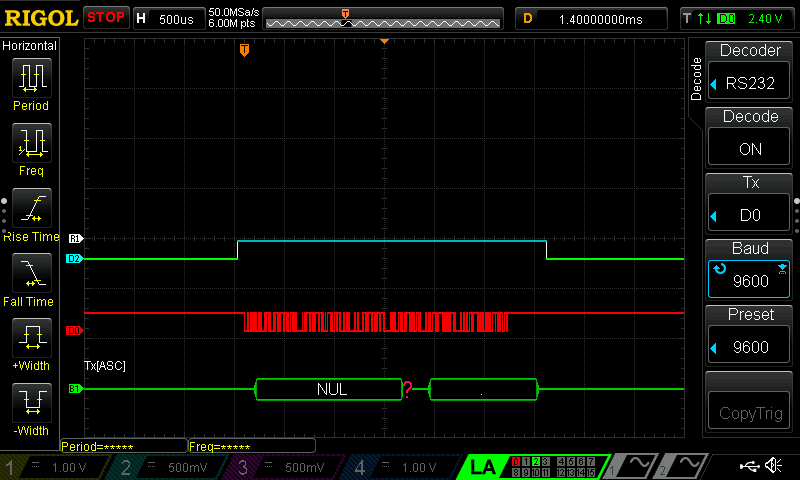
\includegraphics[scale=0.4]{figures/Scope_No_Delay115200.png}
    \caption{When 115200 baudrate is used, the \texttt{usleep()} function seems to sleep too long}
    \label{fig:scope_no_delay115200}
\end{figure}


\newpage

Things start to be really off when an extra byte delay is added in Listing \ref{lst:serial_write_delay} for the 115200 baudrate.
The data is still decent, but instead of an extra $\frac{1}{11520} * 1000000 = 86 \mu S$ that is added to the \texttt{DE} toggling, it seems that an additional $1900 \mu S$ have been added.
This can be seen in Figure \ref{fig:scope_extra_delay115200}.

\begin{figure}[H]
    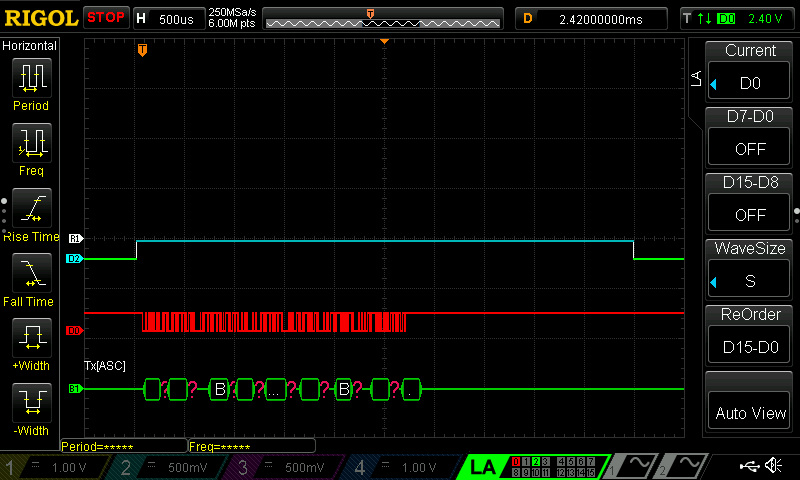
\includegraphics[scale=0.4]{figures/Scope_Extra_Delay115200.png}
    \caption{Things start to be really off when a 1 byte extra delay in Listing \ref{lst:serial_write_delay} is added on a baudrate of 115200}
    \label{fig:scope_extra_delay115200}
\end{figure}

This level of inaccuracy is very problematic because subsystems could potentially start sending their response when the \texttt{DE} pin is high for this long.
This code may actually work and be more accurate on a higher-performance processor such as on the Raspberry Pi 4 or change the Operating System to a  Real Time Operating System.
These are all hypothesis based on the observations made and the performance of the RPI Zero 2. \newline


\textbf{UPDATE:} This problem seems also to be an issue with a much faster CPU.
When sending with a baudrate of 115200 on the Raspberry Pi 4 there is also a delay after the last byte has been sent whilst this is not intentional.


\begin{figure}[H]
    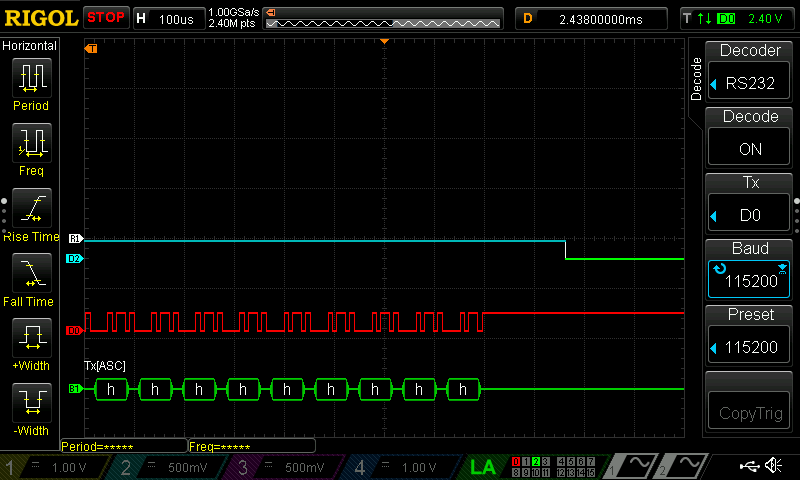
\includegraphics[scale=0.4]{figures/Scope_No_Delay115200_RPI4.png}
    \caption{Even on the Raspberry Pi 4 with a baudrate of 115200 and no extra delay, the \texttt{DE} toggle has a delay}
    \label{fig:scope_no_delay115200_rpi4}
\end{figure}

\newpage
\textbf{SOLUTION:} The old code was switching the \texttt{DE} pin on a software-level and was dependent on the \texttt{usleep()} function making the process unblocked and the Operating System actually scheduling the code as fast as possible to execute the next few lines after \texttt{usleep()} to toggle to \texttt{DE} pin.
In the new code we use \texttt{linux/serial.h} in order to have access to a \texttt{struct serial\_rs485} which we can configure to do the \texttt{DE} toggling in hardware/kernel level.
The example code from the Linux kernel in Listing \ref{lst:rs485_linux} was almost sufficient to get the job done


\begin{lstlisting}[frame=single, caption={Linux RS485 struct to define the \texttt{DE} toggling characteristics in hardware or in the kernel}, captionpos=b, label={lst:rs485_linux}, basicstyle=\small, style=CStyle]
#include <linux/serial.h>

/* Include definition for RS485 ioctls: TIOCGRS485 and TIOCSRS485 */
#include <sys/ioctl.h>

/* Open your specific device (e.g., /dev/mydevice): */
int fd = open ("/dev/mydevice", O_RDWR);
if (fd < 0) {
        /* Error handling. See errno. */
}

struct serial_rs485 rs485conf;

/* Enable RS485 mode: */
rs485conf.flags |= SER_RS485_ENABLED;

/* Set logical level for RTS pin equal to 1 when sending: */
rs485conf.flags |= SER_RS485_RTS_ON_SEND;
/* or, set logical level for RTS pin equal to 0 when sending: */
rs485conf.flags &= ~(SER_RS485_RTS_ON_SEND);

/* Set logical level for RTS pin equal to 1 after sending: */
rs485conf.flags |= SER_RS485_RTS_AFTER_SEND;
/* or, set logical level for RTS pin equal to 0 after sending: */
rs485conf.flags &= ~(SER_RS485_RTS_AFTER_SEND);

/* Set rts delay before send, if needed: */
rs485conf.delay_rts_before_send = ...;

/* Set rts delay after send, if needed: */
rs485conf.delay_rts_after_send = ...;

/* Set this flag if you want to receive data even while sending data */
rs485conf.flags |= SER_RS485_RX_DURING_TX;

if (ioctl (fd, TIOCSRS485, &rs485conf) < 0) {
        /* Error handling. See errno. */
}

/* Use read() and write() syscalls here... */

/* Close the device when finished: */
if (close (fd) < 0) {
        /* Error handling. See errno. */
}
\end{lstlisting}


Please keep in mind that for the Raspberry Pi, the reader has to do a few things such as setting GPIO 17 to an alternative function by loading the \texttt{miniuart-ctsrts.dbto} file from GitHub and in the \texttt{/boot/overlays} directory\footnote{\url{https://forums.raspberrypi.com/viewtopic.php?f=44\&t=241623\#p1473905}}.
The reader has to change the \texttt{/boot.config.txt} file as well (See Subsection \ref{subsec:rpitogglefix}). \newline

As of now there is no extra delay before- or after the message. This is because only delays expressed in milliseconds can be given with the Linux kernel RS485 module and a baudrate of 115200 is quite fast. The least amount of delay, which is 1 millisecond, is quite some time already when one sends on a 115200 baudrate.
Hence why it has been decided that as of now there is no need for an extra delay and we could always add a delay later if data turns out to be transmitted unreliable.

\newpage

\subsection{Raspberry Pi RS485 driver does not toggle \texttt{DE} pin - fix}
\label{subsec:rpitogglefix}

The Raspberry Pi has two UART modules and two different drivers. The main UART module is used to communicate to the on-board Bluetooth module and uses the PL011 driver. The other UART module uses the different miniuart driver and is less stable.
Recently the PL011 driver got updated and has support for hardware control (CTS/RTS) as well which is used by the Linux RS485 driver to toggle the Driver Enable (DE) pin.
However, when we disable Bluetooth by adding the \texttt{dtoverlay=disable-bt} in \texttt{/boot/config.txt} then UART0 should be available to us with the PL011 driver.
However, when one tries to configure the RS-485 driver with the code from Listing \ref{lst:rs485_linux} then we get the output that can be seen in Listing \ref{lst:rpi_error1}.

\begin{lstlisting}[caption={Output when one tries to communicate to \texttt{/dev/ttyAMA0} and Bluetooth is disabled}, captionpos=b, label={lst:rpi_error1}, basicstyle=\small, style=dos]
$ gcc test.c serial.c -o test
$ sudo ./test
[SERIAL] Failed to initialize the RS-485 driver with error 25
\end{lstlisting}

\textbf{SOLUTION:} We were not able to get it working with the Bluetooth driver being disabled and using the PL011 driver on \texttt{/dev/ttyAMA0}. However, we got it partially and very unreliably working by keeping the Bluetooth driver enabled and downloading a compiled dtoverlay script from GitHub\footnote{\url{https://github.com/HiassofT/AtariSIO/tree/master/contrib/rpi}} and place the \texttt{miniuart-ctsrts.dtbo} file in the \texttt{/boot/overlays/} directory.
Once that is done, the reader has to modify the \texttt{/boot/config.txt} file and the bottom few lines should be added

\begin{lstlisting}[caption={If UART is not enabled then add the first line as well in \texttt{/boot/config.txt}}, captionpos=b, label={lst:rpi_fix1}, basicstyle=\small, style=dos]
enable_uart=1
dtoverlay=miniuart-ctsrts
\end{lstlisting}

Since the \texttt{DE} toggling will happen on GPIO17, this pin should be in alternate function 5. We thought it had to be in alternative function 3 but that did not happen to work and might be for the PLA011 driver.
One could verify the alternate function of GPIO 17 with the command below

\begin{lstlisting}[caption={If UART is not enabled then add the first line as well in \texttt{/boot/config.txt}}, captionpos=b, label={lst:rpi_fix1}, basicstyle=\small, style=dos]
$ sudo raspi-gpio get 17
GPIO 17: level=0 fsel=2 alt=5 func=RTS1
\end{lstlisting}

If this is all done then the \texttt{DE} pin used in the Serial library should be toggled by the Linux kernel and the hardware peripheral.
Because of the UART design on the Raspberry Pi it does not happen to work reliable and sometimes for some mysterious reason the \texttt{DE} pin is toggled and immediately toggled again resulting in a very small pulse which can be seen in Figure \ref{fig:RPi_Uart_Bug}


\begin{figure}[H]
    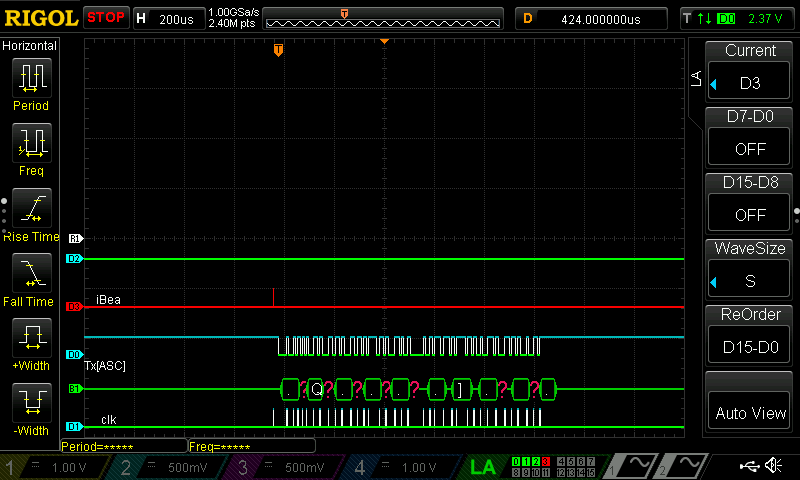
\includegraphics[scale=0.4]{figures/RPi_Uart_Bug.png}
    \caption{Hardware bug of the Raspberry Pi UART design}
    \label{fig:RPi_Uart_Bug}
\end{figure}

For this reason we strongly recommend to use the BeagleBone Black (BBB) as replacement platform for the OBC because it has true UART peripherals which aren't partially reserved for any other on-board device.
It does also run Linux and the Serial library should work more reliably.


%% Use letters for the chapter numbers of the appendices.
\appendix

%\input{appendix-a}

\bibliography{report}




\end{document}
